\documentclass{beamer} 
\usetheme{Madrid} 
% HEADER-BEAMER
% specifically for use in presentations

% a % sign means the rest of the line is ignored
% modify page size and spacing at end

% PREAMBLE
\usepackage{graphicx}
\usepackage{amsmath}
\usepackage{amsfonts}
\usepackage{url}

% format for environments follows
% \newenvironment{name}{starting text}{finishing text}

% matrix and determinant environments follow
\newenvironment{mat}{\left[ \begin{array}}{\end{array} \right]}
\newenvironment{deter}{\left| \begin{array}}{\end{array} \right|}

% controls the way equations are numbered
%\numberwithin{equation}{section}
% format for lists follows
% \begin{list}{label for items}{declarations} items in list \end{list}

% lista, listr, listar, listq are list environments with
% small letters, small roman numerals, arabic numerals and no item labels
\newcounter{ctr}
\newenvironment{lista}{\begin{list}{(\alph{ctr})}%
{\usecounter{ctr}
\setlength{\itemsep}{0mm} \setlength{\topsep}{-2mm}
\setlength{\leftmargin}{3em}}}{\end{list}}

\newcounter{ctr1}
\newenvironment{listr}{\begin{list}{(\roman{ctr1})}%
{\usecounter{ctr1}
\setlength{\itemsep}{0mm} \setlength{\topsep}{-2mm}
\setlength{\leftmargin}{3em}}}{\end{list}}

\newcounter{ctr2}
\newenvironment{listar}{\begin{list}{\arabic{ctr2}.}%
{\usecounter{ctr2}
\setlength{\itemsep}{0mm} \setlength{\topsep}{-2mm}
\setlength{\leftmargin}{3em}}}{\end{list}}

\newenvironment{listq}{\begin{list}{}%
{
\setlength{\itemsep}{0mm} \setlength{\topsep}{-2mm}
\setlength{\leftmargin}{3em}}}{\end{list}}

% environments for an example, examples or exercises follow

\newenvironment{exercises}{\begin{trivlist} \item[]
{\bf Exercises} \begin{enumerate}}{\end{enumerate} \end{trivlist}}


% commands for number sets follow
\newcommand{\NN}{\mathbb{N}}
\newcommand{\ZZ}{\mathbb{Z}}
\newcommand{\QQ}{\mathbb{Q}}
\newcommand{\RR}{\mathbb{R}}
\newcommand{\CC}{\mathbb{C}}
\newcommand{\LL}{\mathbb{L}}

% commands for extra mathematical symbols follow
\newcommand{\half}{\frac{1}{2}}
\newcommand{\third}{\frac{1}{3}}
\newcommand{\quarter}{\frac{1}{4}}
\newcommand{\isimp}{\Leftarrow}
\newcommand{\lsim}{\stackrel{<}{_\sim}}
\newcommand{\gsim}{\stackrel{>}{_\sim}}
\newcommand{\image}{\, {\rm im}\, }
\newcommand{\rank}{\, {\rm r}\, }
\newcommand{\domain}{\, {\rm dom}\, }
\newcommand{\adjoint}{\, {\rm adj}\, }
\newcommand{\signum}{\, {\rm sgn}\, }
\newcommand{\cosec}{\, {\rm cosec}\, }
\newcommand{\cis}{\, {\rm cis}\, }
\newcommand{\sech}{\, {\rm sech}\, }
\newcommand{\cosech}{\, {\rm cosech}\, }
\newcommand{\trace}{\, {\rm trace}\, }
\newcommand{\diag}{\, {\rm diag}\, }
\newcommand{\tri}{\, {\rm tri}\, }
\newcommand{\ud}{\, {\rm d} \kern-.015em }
\newcommand{\const}{\! {\rm const.}\; }


% the following commands need 1 or 2 arguments in { }
\newcommand{\real}[1]{{\rm Re}\left( #1 \right)}
\newcommand{\modulus}[1]{\left| \kern.05em #1 \kern.05em \right|}
\newcommand{\norm}[1]{\left\| \kern.05em #1 \kern.05em \right\|}
\newcommand{\inner}[1]{\left\langle \kern.05em #1 \kern.05em \right\rangle }
\newcommand{\recip}[1]{\frac{1}{#1}}
\newcommand{\seq}[1]{\left( #1 \right)}
\newcommand{\set}[1]{\left\{ #1 \right\} }
\newcommand{\spanof}[1]{\, {\rm span} \left\{ #1 \right\} }
\newcommand{\limit}[2]{\stackrel{\lim }{_{ #1 \to #2 }}}
\newcommand{\maxover}[1]{\stackrel{\max }{_{ #1 }}}
\newcommand{\minover}[1]{\stackrel{\min }{_{ #1 }}}
\newcommand{\dislim}[2]{\renewcommand{\arraystretch}{0.8}
\begin{array}{c}\lim \\ #1 \to #2 \end{array}}
\newcommand{\pdif}[2]{\frac{\partial #1}{\partial #2}}
\newcommand{\pddif}[3]{\frac{\partial^2 #1}{\partial #2 \partial #3}}
\newcommand{\dif}[2]{\frac{\ud #1}{\ud #2}}
\newcommand{\ildif}[2]{{\rm d} #1/{{\rm d} #2 }}
\newcommand{\ilpdif}[2]{\partial #1/{\partial #2 }}
\newcommand{\ilpddif}[3]{\partial^2 #1/{\partial #2 \partial #3}}
\newcommand{\seconddif}[2]{\frac{\ud^2 #1}{\ud #2^2}}
\newcommand{\bm}[1]{\mbox{\protect\boldmath $ #1 $}}
\newcommand{\bmzero}{\mbox{\bf 0}}
\newcommand{\pick}[2]{\renewcommand{\arraystretch}{0.6}
\left( \kern-.4em \begin{array}{c} #1 \\ #2 \end{array} \kern-.4em \right) }
\newcommand{\e}[1]{{\textrm{e}}^{#1}}
\newcommand{\cov}[1]{\, {\rm cov}\left( #1 \right) }
\newcommand{\var}[1]{\, {\rm var}\left( #1 \right) }
\newcommand{\PP}[1]{\mathbb{P}\left( #1 \right)}
\newcommand{\EE}[1]{\mathbb{E} \left( #1 \right)}


%END OF PREAMBLE



\usepackage{subfigure}
\usepackage{ dsfont }
\usepackage{wrapfig}
\usepackage{times}
\usepackage{url}
\usepackage{latexsym}
\usepackage{amsfonts}
\usepackage{arydshln}
\usepackage{graphicx}
\title{Parameter Tuning Off the Grid}
\author{Henry Moss, David Leslie, Paul Rayson}
\date{h.moss@lancaster.ac.uk\\ https://github.com/henrymoss}
\begin{document}
\begin{frame} 
	\titlepage 
\end{frame}	 
\begin{frame}{Plan}
	\begin{enumerate}
		\item Introduce simple NLP task
		\item Grid Search
		\item Random Search
		\item Bayesian Optimisation 
	\end{enumerate}
\end{frame}

\begin{frame}{Generic NLP task}
	\begin{block}{IMDB Data}
		\begin{itemize}
			\item 25,000 positive and 25,000 negative movie reviews.
			\item [$\times$] I'm not a big fan of musicals, although this technically might not qualify as a musical. It was mediocre at best. Hudson seems totally out of kilter in this role. It just didn't work for me. Don't waste your time!
			\item[\checkmark] This is a must-see movie. You will laugh, you will cry, and when it's over you'll wish there were more. Well-written and compelling, this movie draws you in and holds on tight. The casting was perfect, the characters purposeful, and the performances outstanding.
		\end{itemize}
	\end{block}
\end{frame}
\begin{frame}{Generic NLP Model}

	\begin{block}{Model}
		\begin{itemize}
			\item Random Forest Classifier
			\item 5,000 random training examples
			\item BOW of uni-grams, bi-grams and tri-grams.
			\item Use 500 features with highest TF-IDF scores.
			\item 1000 trees
		\end{itemize}
	\end{block}
	\begin{block}{Parameter to Tune}
			\begin{itemize}
				\item max\_features: continuous on $(0,1]$
				\item max\_depth: discrete in $\{1,2,3,4,5\}$
				\item min\_samples\_split: continuous in $(0,0.5]$
				\item min\_samples\_leaf: continuous in $(0,0.5]$
			\end{itemize}
	\end{block}
\end{frame}

\begin{frame}{Approach 1: Grid Search}
	\begin{block}{Grid Search Algorithm}
		\begin{itemize}
			\item Try 3 values for each parameter ($3^4=81$ evaluation):
			\begin{itemize}
				\item max\_features: $\{0.1,0.5,0.9\}$
				\item max\_depth: $\{1,3,5\}$
				\item min\_samples\_split: $\{0.1,0.3,0.5\}$
				\item min\_samples\_leaf: $\{0.1,0.3,0.5\}$
			\end{itemize}
		\item Choose values that give highest 5-fold CV score
		\end{itemize}
	\end{block}

\begin{block}{Chosen Parameter Values}
	\begin{itemize}
		\item max\_features=0.1
		\item max\_depth=1
		\item min\_samples\_split=0.1
		\item min\_samples\_leaf=0.1
	\end{itemize} 
	Providing 68\% Accuracy
\end{block}
\end{frame}
\begin{frame}{Approach 1: Grid Search}
	\begin{block}{Advantages}
		\begin{itemize}
			\item[\checkmark] Simple to understand and implement
			\item[\checkmark] Can exploit prior knowledge of 'good' parameter values
		\end{itemize}
	\end{block}
\begin{block}{Disadvantages}
	\begin{itemize}
		\item[$\times$] Naive exhaustive approach
		\item[$\times$] Computational cost : $n^d$
		\item[$\times$] Setting an effective grid requires prior knowledge
	\end{itemize}
\end{block}
\end{frame}


\begin{frame}{Approach 2: Random Search}
		\begin{block}{Random Search Algorithm}
		\begin{itemize}
			\item Draw a parameter choice:
			\begin{itemize}
				\item max\_features uniformly from $(0,1]$
				\item max\_depth uniformly over $[1,2,3,4,5]$
				\item min\_samples\_split uniformly from $(0,1]$
				\item min\_samples\_leaf uniformly from $(0,1]$
			\end{itemize}
			\item Repeat $n$ times
			\item Choose values that give highest 5-fold CV score
		\end{itemize}
	\end{block}
\end{frame}
\begin{frame}{Approach 2: Random Search}

\begin{block}{}
			\begin{figure}[h]
		\begin{center}
			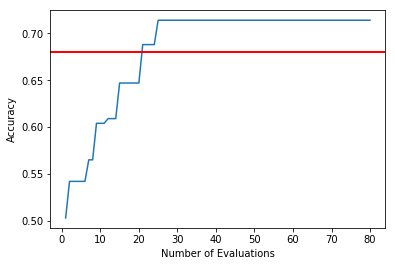
\includegraphics[height=5cm]{single_random}
		\end{center}
	\end{figure}
	Accuracy of the best found parameter values from random-search. The red line represents the performance found by grid-search.
\end{block}
\end{frame}
\begin{frame}
		\begin{block}{}
		Look at performance over 50 runs of random search
		
		\begin{figure}[h]
			\begin{center}
				\subfigure[]{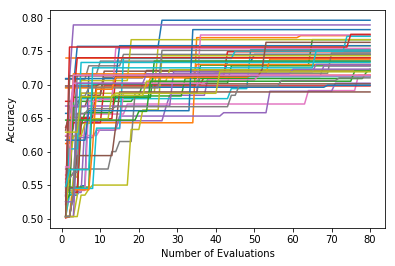
\includegraphics[height=3.5cm]{many_random}}
				\subfigure[]{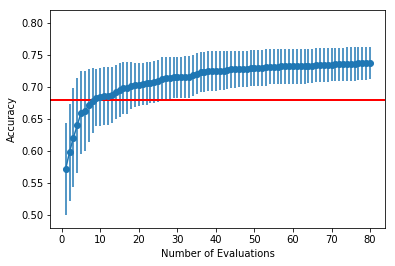
\includegraphics[height=3.5cm]{many_random2}}
			\end{center}
		\end{figure}
	\end{block}
\end{frame}

\begin{frame}{Approach 2: Random Search}
	\begin{block}{Advantages}
	\begin{itemize}
		\item[\checkmark] Equally simple to understand and even easier to implement
		\item[\checkmark] Adding non-important parameters doesn't effect performance
		\item[\checkmark] Freedom to choose computational budget
	\end{itemize}
\end{block}
\begin{block}{Disadvantages}
	\begin{itemize}
		\item[$\times$] Harder to retain reproducibility
		\item[$\times$] Small chance of not finding a 'good' solution
		\item[$\times$] Could repeat evaluations of poorly performing parameter choices
	\end{itemize}
\end{block}
\end{frame}

\begin{frame}{Approach 2: Random Search}
	\begin{block}{Intuition 1: Evaluate each parameter at more places $^1$}
		\begin{figure}[h]
		\begin{center}
			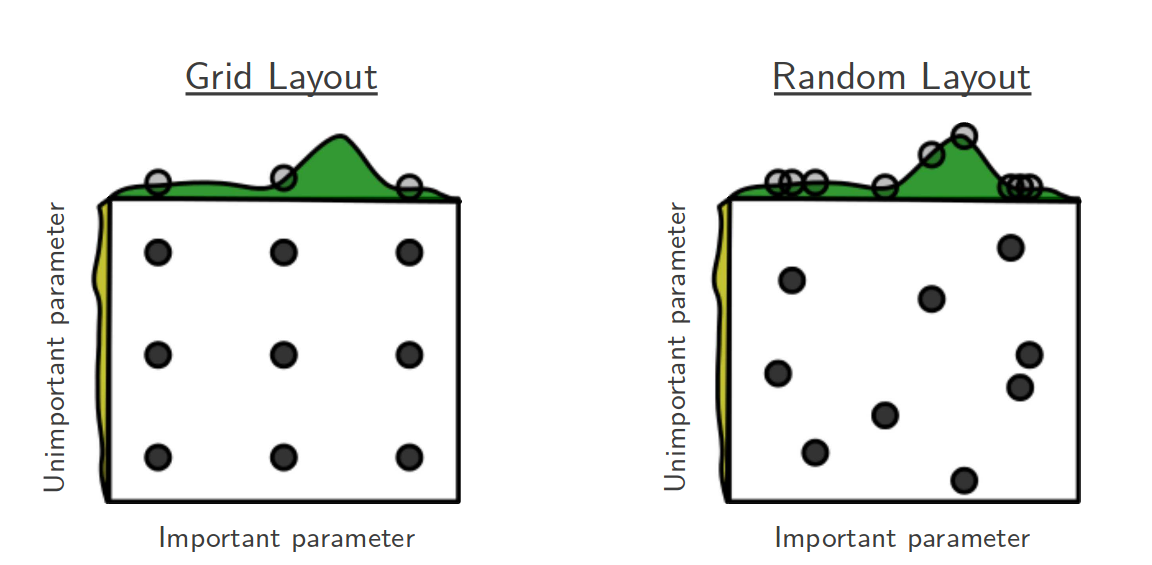
\includegraphics[height=5cm]{gris_random_bergstra}
		\end{center}
	\end{figure}
	\end{block}
\end{frame}

\begin{frame}{Approach 2: Random Search}
	\begin{block}{Intuition 2: High probability of finding "good" parameter values$^2$}
\begin{itemize}
	\item Consider the region $R$ containing the optimum parameter choice and the surrounding $5\%$ of parameter space.
	\item Each of $n$ random evaluation has a $5\%$ chance of being in $R$
	\item $p=prob(At\  least\ one\ point\ is\ in\ R)=1-(1-0.005)^n$
	\item For $n\geq60$ $p>0.95$
\end{itemize}
	\end{block}
\end{frame}

\begin{frame}{An Aside: Clever Searching for Optima$^5$}
	\begin{block}{}
		Consider Trying to find the minimum of $f(x)=(6x-2)^2sin(12x-4)$
		
	
	\begin{figure}[h]
		\begin{center}
			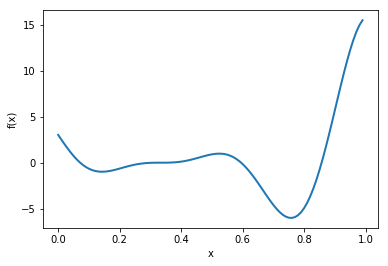
\includegraphics[height=4cm]{forest}
		\end{center}
	\end{figure}
Using as few function evaluations as possible
	\end{block}
\end{frame}

\begin{frame}{An Aside: Clever Searching for Optima$^5$}
	\begin{block}{}
	Suppose we make evaluations at 0,0.5 and 1
	
	
	\begin{figure}[h]
		\begin{center}
			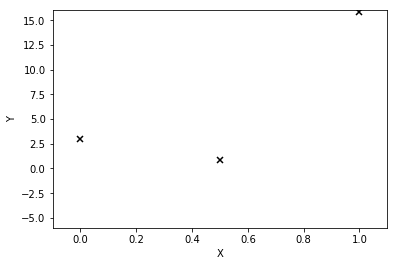
\includegraphics[height=4cm]{points}
		\end{center}
	\end{figure}
	Where should we next evaluate? \\
	What would grid or random search do?
\end{block}
\end{frame}

\begin{frame}{An Aside: Clever Searching for Optima$^5$}
	\begin{block}{}
	Possible functions that pass through the observed points
	
	
	\begin{figure}[h]
		\begin{center}
			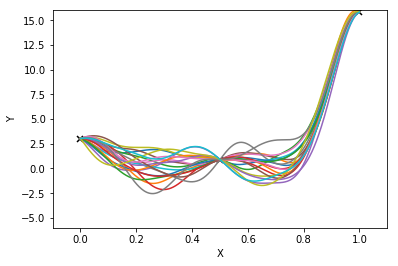
\includegraphics[height=4cm]{functions}
		\end{center}
	\end{figure}
	Where should we next evaluate?
\end{block}
\end{frame}

\begin{frame}{An Aside: Clever Searching for Optima$^5$}
	\begin{block}{}
	We can summarize this belief by fitting a Gaussian process

	\begin{figure}[h]
		\begin{center}
			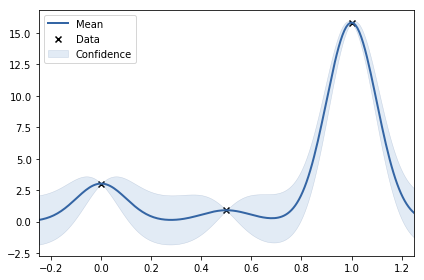
\includegraphics[height=4cm]{GP}
		\end{center}
	\end{figure}
	Where should we next evaluate?\\
	Do we want to explore?\\
	or exploit?\\
\end{block}
\end{frame}

\begin{frame}{An Aside: Clever Searching for Optima$^5$}
	\begin{block}{}
		Compare our statistical model with the truth
		
	\begin{figure}[h]
	\begin{center}
		\subfigure[Fitted Gaussian Process]{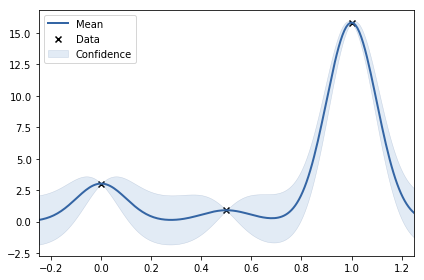
\includegraphics[height=3.5cm]{GP}}
		\subfigure[Truth]{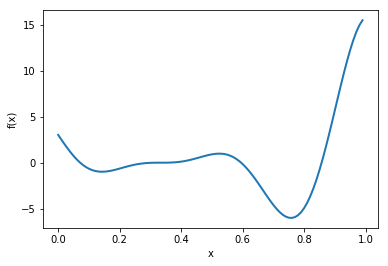
\includegraphics[height=3.5cm]{forest}}
	\end{center}
\end{figure}
	\end{block}
\end{frame}

\begin{frame}{An Aside: Clever Searching for Optima$^5$}
	\begin{block}{}
	We choose the next evaluation by maximizing an acquisition function
	
	\begin{figure}[h]
	\begin{center}
		\subfigure[Fitted Gaussian Process]{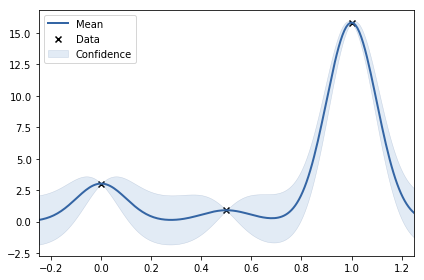
\includegraphics[height=3.5cm]{GP}}
		\subfigure[Acquisition Function]{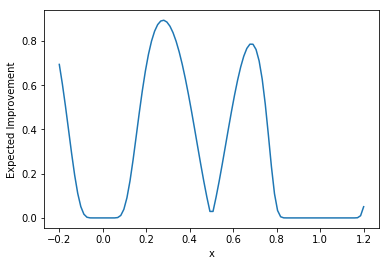
\includegraphics[height=3.5cm]{EI}}
	\end{center}
\end{figure}
	This procedure is known as Bayesian Optimization (BO)
\end{block}
\end{frame}
\begin{frame}{An Aside: Full BO implementation$^6$}
	\begin{block}{}
		Model after 4 initial points and 1 evaluation chosen by BO
			\begin{figure}[h]
			\begin{center}
				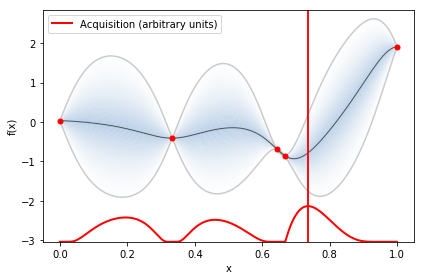
\includegraphics[height=5cm]{BO1}
			\end{center}
		\end{figure}
	\end{block}
\end{frame}
\begin{frame}{An Aside: Full BO implementation$^6$}
	\begin{block}{}
		Model after 4 initial points and 2 evaluations chosen by BO
		\begin{figure}[h]
			\begin{center}
				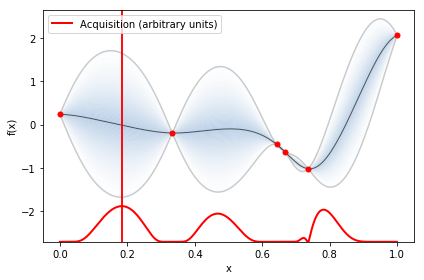
\includegraphics[height=5cm]{BO2}
			\end{center}
		\end{figure}
	\end{block}
\end{frame}
\begin{frame}{An Aside: Full BO implementation$^6$}
	\begin{block}{}
		Model after 4 initial points and 3 evaluations chosen by BO
		\begin{figure}[h]
			\begin{center}
				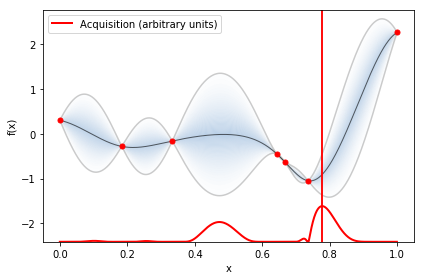
\includegraphics[height=5cm]{BO3}
			\end{center}
		\end{figure}
	\end{block}
\end{frame}
\begin{frame}{An Aside: Full BO implementation$^6$}
	\begin{block}{}
		Model after 4 initial points and 4 evaluations chosen by BO
		\begin{figure}[h]
			\begin{center}
				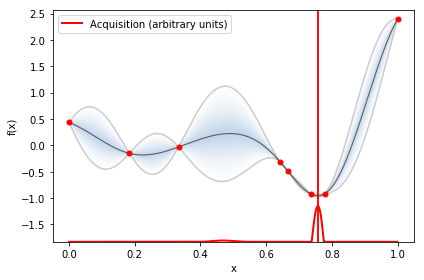
\includegraphics[height=5cm]{BO4}
			\end{center}
		\end{figure}
	\end{block}
\end{frame}
\begin{frame}{Approach 3: Bayesian Optimization (BO)}
	\begin{block}{}
		\begin{figure}[h]
			\begin{center}
				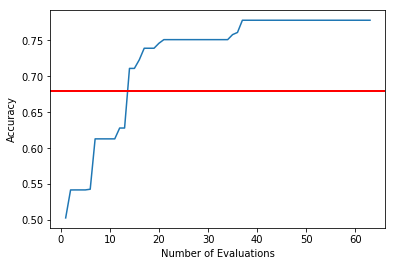
\includegraphics[height=5cm]{single_BO}
			\end{center}
		\end{figure}
		Accuracy of the best found parameter values from BO. The red line represents the performance found by grid-search.
	\end{block}
\end{frame}
\begin{frame}{Approach 3: Bayesian Optimization (BO)}
			\begin{block}{}
		Look at performance over 50 runs of BO
		
		\begin{figure}[h]
			\begin{center}
				\subfigure[BO for 25 evaluations]{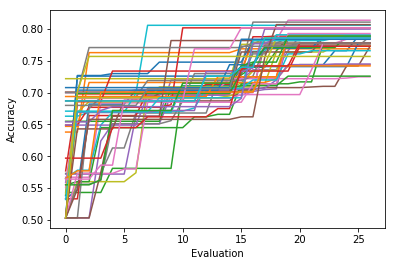
\includegraphics[height=3.5cm]{many_BO}}
				\subfigure[Random-search for 81 evaluations]{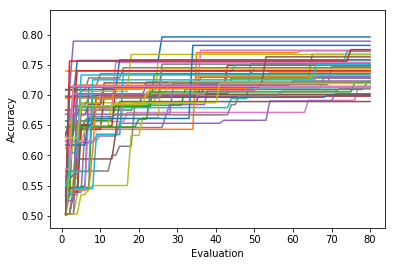
\includegraphics[height=3.5cm]{many_random3}}
			\end{center}
		\end{figure}
	\end{block}
\end{frame}
\begin{frame}{Approach 3: Bayesian Optimization (BO)}
	\begin{block}{}
		Look at performance over 50 runs of BO
		
		\begin{figure}[h]
			\begin{center}
				\subfigure[BO for 25 evaluations]{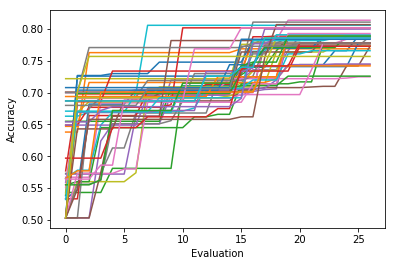
\includegraphics[height=3.5cm]{many_BO}}
				\subfigure[Random-search for 25 evaluations]{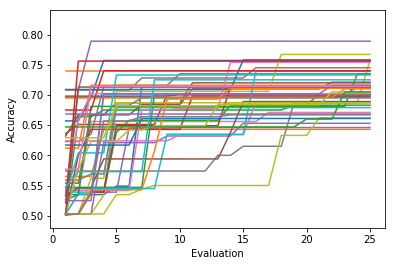
\includegraphics[height=3.5cm]{many_random4}}
			\end{center}
		\end{figure}
	\end{block}
\end{frame}
\begin{frame}{Approach 3: Bayesian Optimization (BO)}
		\begin{block}{Advantages}
		\begin{itemize}
			\item[\checkmark] Efficient 
			\item[\checkmark] Doesn't revisit bad parameter values
			\item[\checkmark] Fully black-box
		\end{itemize}
	\end{block}
	\begin{block}{Disadvantages}
		\begin{itemize}
			\item[$\times$] More complicated
			\item[$\times$] Computational cost grows cubically in $n$
		\end{itemize}
	\end{block}
\end{frame}

\begin{frame}{Further Questions}
	\begin{block}{}
		\begin{itemize}
			\item \textbf{Is 5-fold CV appropriate for effective tuning?} \\
			We say it often is not \textit{https://arxiv.org/abs/1806.07139}
			\item \textbf{Can we adaptively choose how to partition our data as part of BO?} \\
			We think so, watch this space!
					
		\end{itemize}
	\end{block}
\end{frame}
\begin{frame}
	\begin{block}{References}
		\begin{enumerate}
			\item \textbf{Intuition 1:} A blog post by Alice Zheng \textit{https://www.oreilly.com/ideas/evaluating-machine-learning-models/page/5/hyperparameter-tuning}
			\item \textbf{Intuition 2:} Bergstra and Bengio, Random search for hyper-parameter optimization, Journal of Machine Learning Research, 2012.
			\item \textbf{Bayesian Optimization Summary:} Snoek, Larochelle, and Adams, Practical bayesian optimization of machine learning algorithms, Advances in neural information processing systems, 2012.
			\item \textbf{Gaussian Process Introduction:} Williams and Rasmussen, Gaussian processes for machine learning, MIT Press, 2006.
			\item \textbf{Python Package for Gaussian Processes:} GPy, \textit{https://sheffieldml.github.io/GPy/} 
			\item \textbf{Python Package for BO:} GPyOpt, \textit{https://sheffieldml.github.io/GPyOpt/}
		\end{enumerate}
	\end{block}
\end{frame}

\end{document} 